\subsection*{Banktilgang}
\begin{figure}[!htb]
\centering
\begin{minipage}{0.4\textwidth}
	Det første du må gjøre, er å levere inn en egenerklæring til økonomiansvarlig i HS. Det ligger et skjema på ntnui.no som fylles ut med kopi av gyldig legitimasjon. Se gjerne bildet til høyre. \\
	Deretter må du besøke \href{https://www.danskebank.no/nb-no/bedrift/smaabedrifter/nettbank/pages/identifisering.aspx}{danskebank.no og legitimere deg med BankID}. Den enkleste måten å finne frem på, er å google \emph{``danske bank legitimering''}. \\ \\
Når alt det er gjort, vil økonomiansvarlig opprette en bruker hos banken, og du vil finne kodebrikke og midlertidig passord i posthylla etter 3-4 virkedager.
\end{minipage}
\begin{minipage}{0.5\textwidth}
	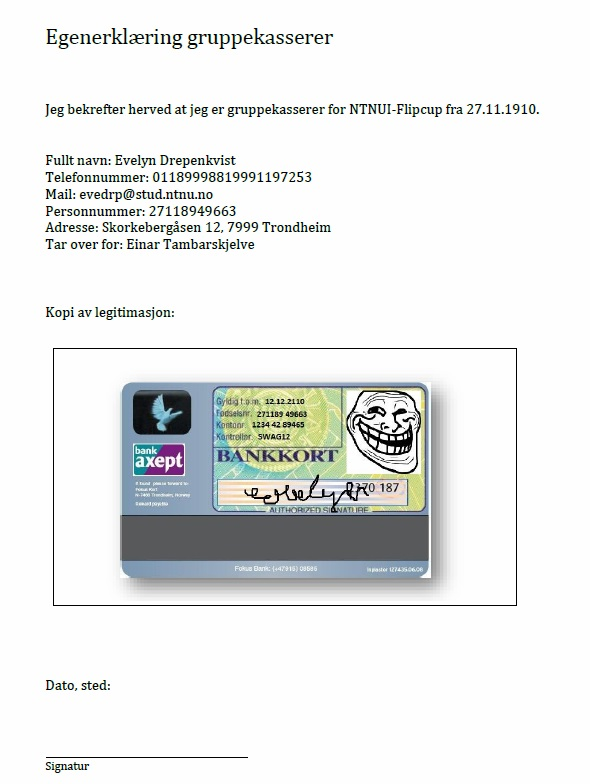
\includegraphics[scale=0.5]{bildr/egenerklaring.jpg}
\end{minipage}
\end{figure}